\documentclass[a4paper, 12pt]{article}

% a nice font
\usepackage{kpfonts}

% basic text stuff
\usepackage[utf8]{inputenc}
\usepackage[T1]{fontenc}

\usepackage{tikz} % main tikz package

\usetikzlibrary{external}
\tikzexternalize[prefix=compiled_figures] % prefix sets where to store figures

% for a nicer colorscheme
\definecolor{blue}{rgb}{0.38, 0.51, 0.71} %glaucous, 97,130,181, #6182B5
\definecolor{darkblue}{RGB}{17, 42, 60} % 112A3C
\definecolor{red}{RGB}{175, 49, 39} % AF3127

\definecolor{orange}{RGB}{217, 156, 55} % D99C37
\definecolor{green}{RGB}{144, 169, 84} % 90A954
\definecolor{palegreen}{RGB}{197, 184, 104} % C5B868

\definecolor{yellow}{RGB}{250, 199, 100} % FAC764
\definecolor{brokenwhite}{RGB}{218, 192, 166} % DAC0A6
\definecolor{brokengrey}{rgb}{0.77, 0.76, 0.82} % {196,194,209}, C4C2D1


\usetikzlibrary{arrows}
\usetikzlibrary{3d}
\usetikzlibrary{calc}

\begin{document}
    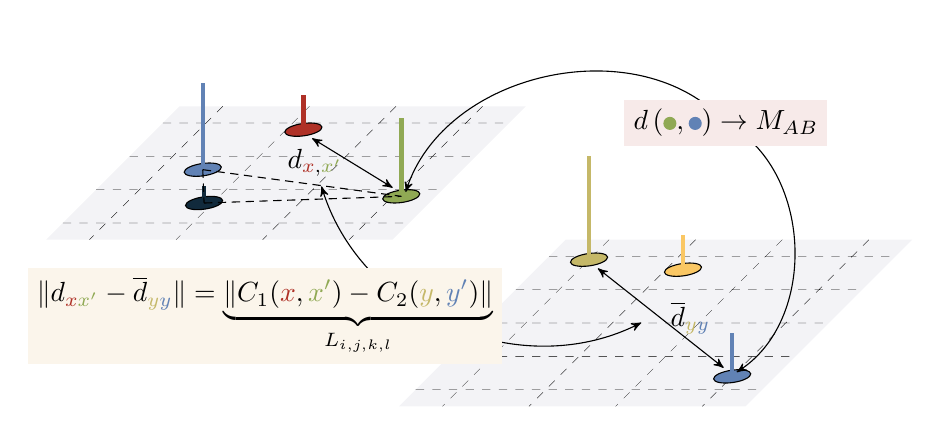
\begin{tikzpicture}[scale=1.1,>=stealth',tips=proper]
                \coordinate (a) at (0.5, 0, 1.4);
                \begin{scope}[canvas is xz plane at y = 0]
                    \fill[brokengrey!20] (-0.5, -0.5) rectangle (3.5, 3.5);
                    \draw[dashed, ultra thin] (-0.5, -0.5) grid (3.5, 3.5);

                    \fill[brokengrey!20] (5.5, 3.5) rectangle (9.5, 8.5);
                    \draw[dashed, ultra thin] (5.5, 3.5) grid (9.5, 8.5);
                \end{scope}

                \begin{scope}[canvas is xz plane at y = 0]
                	\draw[fill=blue] (0.5,1.4) circle (0.2);
                	\draw[fill=darkblue] (0.9,2.4) circle (0.2);
                	\draw[fill=red] (1.2,0.2) circle (0.2);
                	\draw[fill=green] (3.1,2.2) circle (0.2);
                	\draw[fill=palegreen] (6.0,4.1) circle (0.2);
                	\draw[fill=yellow] (7.2,4.4) circle (0.2);
                	\draw[fill=blue] (9.0,7.6) circle (0.2);
                \end{scope}

                \coordinate (blue) at (0.5, 0.0,1.4);
                \draw[ultra thick, blue] (0.5, 0.0,1.4) -- (0.5, 1.0,1.4);
                \coordinate (darkblue) at (0.9, 0.0,2.4);
                \draw[ultra thick, darkblue] (0.9, 0.0,2.4) -- (0.9, 0.2,2.4);
                \coordinate (red) at (1.2, 0.0,0.2);
                \draw[ultra thick, red] (1.2, 0.0,0.2) -- (1.2, 0.4,0.2);
                \coordinate (green) at (3.1, 0.0,2.2);
                \draw[ultra thick, green] (3.1, 0.0,2.2) -- (3.1, 0.9,2.2);
                \coordinate (palegreen) at (6.0, 0.0,4.1);
                \draw[ultra thick, palegreen] (6.0, 0.0,4.1) -- (6.0, 1.2,4.1);
                \coordinate (yellow) at (7.2, 0.0,4.4);
                \draw[ultra thick, yellow] (7.2, 0.0,4.4) -- (7.2, 0.4,4.4);
                \coordinate (blue2) at (9.0, 0.0,7.6);
                \draw[ultra thick, blue] (9.0, 0.0,7.6) -- (9.0, 0.5,7.6);

                \draw[densely dashed] (blue) -- (darkblue);
                \draw[densely dashed] (blue) -- (green);
                \draw[densely dashed] (darkblue) -- (green);

                \draw[bend right = -60, <->] ($(green)+(0.05, 0.05, 0)$) to (6,0) to ($(blue2)+(0.05,0.05,0.)$);
                \node[fill=red!10] (distance) at (6, 0) {$d\left(\tikz\draw[green,fill=green] (0,0) circle (.5ex);, \tikz\draw[blue,fill=blue] (0,0) circle (.5ex); \right) \rightarrow M_{AB} $};

                \draw[<->] ($(red)+(0.1, -0.1, 0)$) -- ($(green) + (-0.1, 0.1, 0)$)  node (middle1) [midway, left] {$d_{{\color{red}x},{\color{green}x'}}$};
                \draw[<->] ($(palegreen)+(0.1, -0.1, 0)$) -- ($(blue2) + (-0.1, 0.1, 0)$) node (middle2) [midway, left] {} node [midway, right] {$\overline{d}_{{\color{palegreen}y}{\color{blue}y}}$};

                \draw[bend right=50, <->] (middle1) to (middle2) node [fill=orange!10, below left,yshift=20, xshift=-50, rotate = 0] {$\| d_{{\color{red}x}{\color{green}x'}} - \overline{d}_{{\color{palegreen}y}{\color{blue}y}} \| = \underbrace{\| C_1({\color{red}x}, {\color{green}x'}) - C_2({\color{palegreen}y}, {\color{blue}y'})\|}_{L_{i,j,k,l}}$};
            \end{tikzpicture}
\end{document}
